\documentclass[conference]{acmsiggraph}

\usepackage{mdwlist}
\usepackage{graphics}
\usepackage{graphicx}
\usepackage{listings}
\usepackage{enumitem}
\usepackage[utf8]{inputenc}

%%%%%%%%%%%%%%%
% Information %
%%%%%%%%%%%%%%%

\title{Plant Modeling Using Environmental Parameters}

\author{
  Andre Philipp\thanks{e-mail:philipp.andy@gmail.com}
  \qquad
  Andy Spencer\thanks{e-mail:andy753421@ucla.edu}
  \qquad
  Haakon Garseg Mørk\thanks{e-mail:haakongmork@gmail.com}
  \\
  University of California, Los Angeles \\
  CS275 Artificial Life for Computer Graphics and Vision
}

\pdfauthor{Andre Philipp, Andy Spencer, Haakon Garseg Mørk}

\keywords{radiosity, global illumination, constant time}

%%%%%%%%%%%%
% Document %
%%%%%%%%%%%%

% Proposal
% --------
% Team:
%
%   Andy Philipp <philipp.andy@gmail.com>
%   Andy Spencer <andy753421@ucla.edu>
%   Haakon Garseg Moerk <haakongmork@gmail.com>
%
% Title:
%
%   Plant Modeling Using Environmental Parameters
%
% Summary:
%
%   The project will focus on modeling natural looking plants using
%   simulated environment parameters to control growth and evolution of
%   different plant species. Genetic algorithms or other evolutionary
%   techniques will be used to evolve plant suitable for growth in various
%   environments.
%
% Potential environmental conditions:
%
%   - Availability of water
%   - Amount of sunlight
%   - Soil conditions
%   - Growth elevation
%
% Potential plant species parameters:
%
%   - Rate of water loss
%   - Food and water storage capability
%   - Total mass/volume
%   - Crown height
%   - Leaf area
%   - Root structures

% Project submission
% ------------------
% We need to make web page containing:
%
%   1. The project abstract
%   2. A link to the paper
%   3. Links to any demos or videos
%
% The paper should be in conference format:
%
%   1. We can use two-column style with, e.g.:
%        a) references,  b) technical description,
%        c) results,     d) conclusions
%   2. It should be medium length, 5 pages is fine.

% Outline
% -------
% 1. Introduction
% 2. Architecture
% 3. Plant System
% 4. Genetics
% 5. Results
% 6. Conclusions

\begin{document}

%%%%%%%%%%%%%%
% Title Page %
%%%%%%%%%%%%%%

\maketitle

\begin{abstract}

The project will focus on modeling natural looking plants using simulated
environment parameters to control growth and evolution of different plant
species. Genetic algorithms or other evolutionary techniques will be used to
evolve plant suitable for growth in various environments.

Potential environmental conditions:

\begin{itemize*}
  \item Availability of water
  \item Amount of sunlight
  \item Soil conditions
  \item Growth elevation
\end{itemize*}

Potential plant species parameters:

\begin{itemize*}
  \item Rate of water loss
  \item Food and water storage capability
  \item Total mass/volume
  \item Crown height
  \item Leaf area
  \item Root structures
\end{itemize*}

\end{abstract}

\keywordlist

%%%%%%%%%%%%
% Content %
%%%%%%%%%%%%

\section{Introduction}

Karl Sims introduced Panspermia in 1990.

LSystem

We closely examined different existing frameworks that we considered using for
our project. The two frameworks that were the best candidates was
OpenAlea\cite{openalea} and Algorithmic Botany\cite{abotany}.

\section{Software Architecture}

The software was implemented using Java and OpenGL for drawing. The top-level
architecture can be divided into two main categories: plant simulation using
L-Systems and the graphical user interface.

\subsection{Plants}

The L-Systems are implemented in the LSystem and LRule classes, which are
responsible for storing the production rules associated with each plant and
iterating the plants phenotype as the plant grows throughout the simulation. The
Gene and Plant classes store representations of each living plant. The Gene
class represents the plant genotype as a combination of the L-System production
rules along with additional information such as stem and leaf size, stem and
flower colors, the number of seeds produced, and the age at which the plant
matures. Each individual plants phenotype is represented using the Plant class
and contains it's X/Y position and orientation inside the world, along with the
current age and a L-System string (L-String) representing the plants current
shape. The Plant class is also responsible for calculating each individual
plants fitness values at the end of each simulation step.

\subsection{User Interface}

The graphical interface is comprised of the Main class, a Drawer class, and a
Video utility class for recording screen captures of the simulation. The Main
class receives user input to control the plant simulation. It also contains the
environmental parameters and invokes the plant growth and fitness functions. The
Drawer class receives a list of plants from the Main class and displays them to
the user. The graphical interfaces also provides convenient controls for each of
the environmental parameters so that they can be tuned while the simulation is
executing.

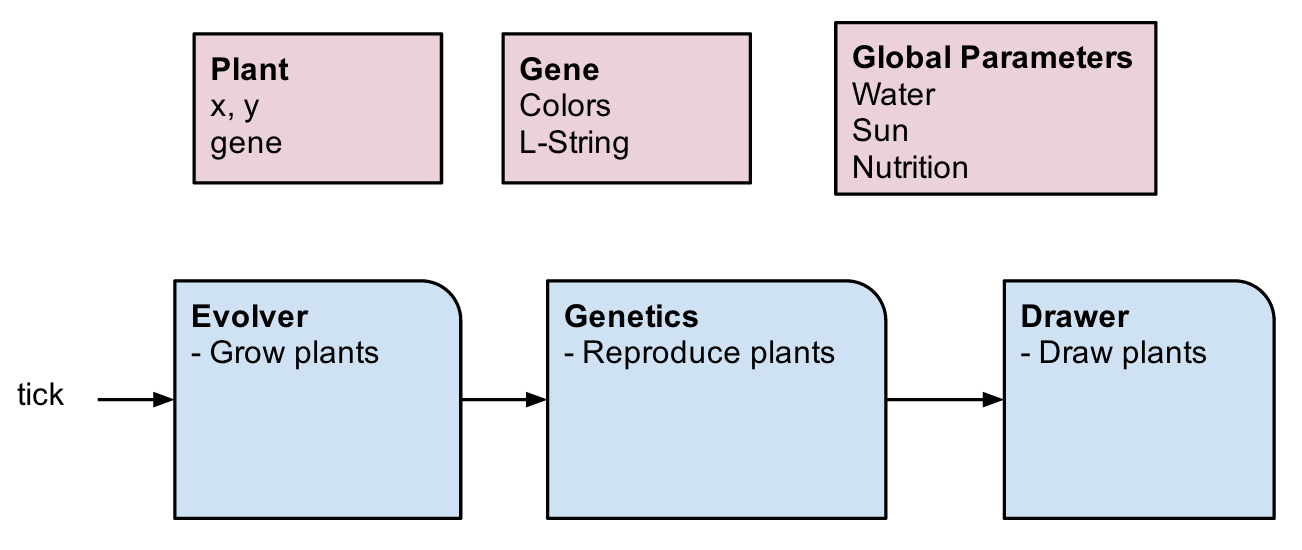
\includegraphics[width=\columnwidth]{images/architecture.png}

\section{Plant Simulation}

Each plant in our environment contains a string of symbol (which we call an
"L-String") representing the plants current shape and size. Each symbol can
represent a stem segment, a flower, a leaf, etc. The plants genotype contains a
set of production rules that govern the growth and development of the plant.
When the plant grows, the production rules are used to replace symbols in the
plants current L-String with sequences of tokens to produces a larger and more
complex plant.

\subsection{L-System Genotypes}

We implemented a modified variant of L-Systems where a replacement probability
is included in addition to the matching and replacement parts of each production
rule. The possible values for each symbol in our rules are as follows:

\begin{description}[leftmargin=!,labelindent=0.2in,labelwidth=0.1in]
  \item[G]   grow a stem segment
  \item[F]   grow a flower at the current position
  \item[L]   grow a leaf at the current position
  \item[X]   does not correspond to any drawing action and is used to control
             the evolution of the curve.\cite{lsystems}
  \item[n, e, s, w] \hfill \\
             bend plants growing direction either north, east, south or west.
             The angle is dependent on the genes angle.
  \item[{[}] push matrix, the current position and angle of growth are saved.
  \item[{]}] pop matrix, the position and angle from he corresponding {]} are
             restored.
\end{description}

Using the push and pop symbols, {[} and {]}, the plant can grow branches in
different directions. For example, a north -- south Y shape can be grown using
the string: \[ G [ s G ] [ n G ] \]

An example of a plant at first generation:

\begin{description}[leftmargin=!,labelindent=0.2in,labelwidth=0.4in]
  \item[Angle] 15 degrees
  \item[Axiom] $ X $
  \item[Rules] $ X \rightarrow Gs[[G]eX]nG[wGX]G \\
                 G \rightarrow GG $
\end{description}

Notice that this plant will not start with flowers ($F$) or leaves ($L$).

\subsection{Simulation}

The simulation of the plant environment is governed by ticks. During each tick,
each of the currently living plant objects becomes older. We wanted to have a
similar approach to have plants grow in the real world. Consequently, during the
first 4 ticks the plant grows as a seed under ground. On the fifth tick it
starts growing above ground. When the seventh tick is reached, the plant becomes
mature and grows flowers and leaves, if the plants genotype is capable of it.
The plant object then spreads it seeds within a certain radius. When the season
is over, the plant dies, but it's children grows up with either the same gene,
or a mutation of the gene.

\section{Genetic Algorithms}

In plant biology, reproduction is divided into two categories: asexual
reproduction and sexual reproduction. In our project we chose to use asexual
reproduction to avoid implementing genetic crossover and recombination. Each of
our plants is initially a clone of it's parent, however there is a probability
that mutations will be introduced during the cloning process.\cite{plantrepo}

In our simulation, the seasons are divided into ticks, at the seventh tick of
the season, the plants are considered mature and will produce seeds. After the
plants have reproduced and the season has ended all the existing plants are
removed and the new child plants are given a chance to grow.

\subsection{Mutation}

When each plant produces seeds, the seed may mutation in several different
ways. Mutation is controlled based on a mutation probability global to all the
plants, if the seed is chosen to be mutated it will change randomly in one of
the following ways:

\begin{description}
  \item[Stem color]   \hfill \\
    The plants stem color is changed randomly, the stem color color is also used
    for the plants leaves.
  \item[Flower color] \hfill \\
    The plants flower color is changed randomly. Both the stem color and flower
    color are only used for display and can be used to help differentiate plants
    of different species.
  \item[Stem width]   \hfill \\
    The diameter of the plants stem is changed. Upper and lower limits are
    imposed and a width is randomly chosen from within the range.
  \item[Leaf size]    \hfill \\
    The length of each leaf is changed. Upper and lower limits are used. The
    leaf shape is fixed for drawing purposes.
  \item[Growth rules] \hfill \\
    The L-System productions used to control the plants growth are changed. The
    plant may become either more or less complex.
\end{description}

\subsubsection{Growth rule mutation}

We want to simulate subtle changes in the gene as the mutation isn't suppose to
be extreme in any ways. Gene mutation occurs by choosing one of the production
rules and then mutation the replacement side of the rule. A symbol is randomly
chosen from the replacement to be mutated.

The mutation can either be that the symbols is simply deleted, or that is then
replaced with a sequences from a predefined set of possible mutations.

The replacement sequences we used are logically divided into several logical
groups, however these divisions are just for convenience and are not used by the
mutation algorithm.

\begin{description}[leftmargin=!,labelindent=0.2in,labelwidth=0.5in]
  \item[Stems]   $G,~~xG,~~[G],~~[xG]$
  \item[Flowers] $F,~~xF,~~[F],~~[xF]$
  \item[Leaves]  $L,~~xL,~~[L],~~[xL]$
  \item[Other]   $[X],~~xX$
\end{description}

Note that in in each of the replacements, `x' is substituted with a random
direction to grow, i.e. `n', `e', `s' or `w'.

\subsection{Fitness}

% // Water
% wfit  -= surfaceArea   * water;      // Large surface area looses water
% wfit  += stemRatio     * water;      // Large stems can store water
% 
% // Sun
% sfit  += surfaceArea*2 * sun;        // Large leaves gather more light
% sfit  += stemCount     * sun;        // Taller plants have an advantage
% 
% // Nutrition
% nfit  -= stemRatio     * nutrition;  // Large plants require more nutrients
% nfit  -= surfaceArea   * nutrition;  // Large plants require more nutrients
% nfit  -= stemCount     * nutrition;  // Large plants require more nutrients

\subsubsection{Environmental parameters}

There are three basic environmental parameters which has an effect on the
plants. The amount of sun (0-100\%), water (0-100\%) and the nutrition available
in the ground.

\section{Conclusion}

%%%%%%%%%%%%%%
% References %
%%%%%%%%%%%%%%

\bibliographystyle{acmsiggraph}
\bibliography{paper}

\end{document}
